\documentclass{article}
\usepackage{tikz}
\usetikzlibrary{arrows.meta,positioning,calc,shapes.geometric}
\pagestyle{empty}
\begin{document}
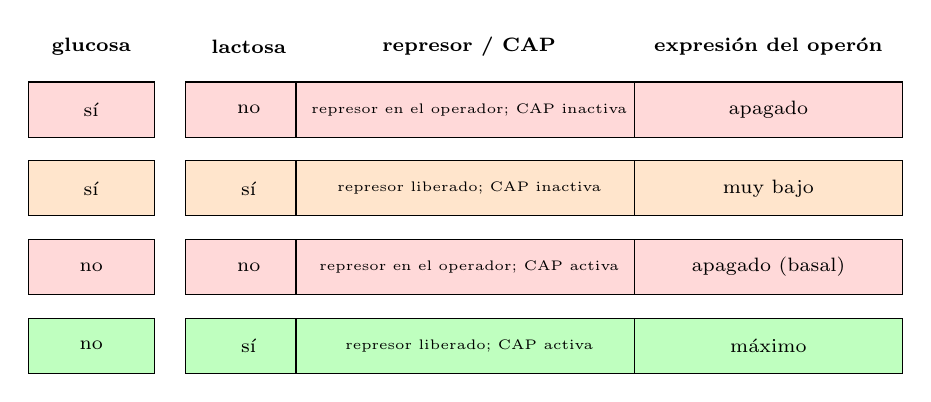
\begin{tikzpicture}

\node[font=\bfseries\scriptsize] at (1.4,4.3) {glucosa}; \node[font=\bfseries\scriptsize] at (3.4,4.3) {lactosa}; \node[font=\bfseries\scriptsize] at (6.2,4.3) {represor / CAP}; \node[font=\bfseries\scriptsize] at (10.0,4.3) {expresión del operón};
\foreach \y/\g/\l/\r/\e/\c in {3.5/sí/no/represor en el operador; CAP inactiva/apagado/red!15, 2.5/sí/sí/represor liberado; CAP inactiva/muy bajo/orange!20, 1.5/no/no/represor en el operador; CAP activa/apagado (basal)/red!15, 0.5/no/sí/represor liberado; CAP activa/máximo/green!25} {
  \node[draw, fill=\c, minimum width=1.6cm, minimum height=0.7cm, font=\scriptsize] at (1.4,\y) {\g};
  \node[draw, fill=\c, minimum width=1.6cm, minimum height=0.7cm, font=\scriptsize] at (3.4,\y) {\l};
  \node[draw, fill=\c, minimum width=4.4cm, minimum height=0.7cm, font=\tiny] at (6.2,\y) {\r};
  \node[draw, fill=\c, minimum width=3.4cm, minimum height=0.7cm, font=\scriptsize] at (10.0,\y) {\e};}

\end{tikzpicture}
\end{document}
